% Gallery figure source
% Summary: Species-level reticulation modes. Hybridization forms a hybrid descendant lineage, introgression moves alleles or tracts through hybridization and backcrossing while both species persist, and horizontal gene transfer moves DNA across species boundaries without reproductive hybridization.
\documentclass[tikz,border=6pt]{standalone}
% Shared color palette
\usepackage[T1]{fontenc}
\usepackage[utf8]{inputenc}
\usepackage{lmodern}
\usepackage{microtype}
\usepackage{amsmath,amssymb,mathtools}
\usepackage{xcolor}
\usepackage{tikz}
\usetikzlibrary{arrows.meta,positioning,calc,fit,backgrounds,decorations.pathreplacing,shapes.geometric,shadows.blur}

\definecolor{mainblue}{RGB}{42,85,132}
\definecolor{deepgreen}{RGB}{30,105,70}
\definecolor{burntorange}{RGB}{190,90,25}
\definecolor{softgray}{RGB}{245,246,248}
\definecolor{darkgray}{RGB}{70,70,70}
\definecolor{violet}{RGB}{110,70,150}

\newcommand{\given}{\,|\,}
\newcommand{\Ne}{N_{e}}
\newcommand{\ARG}{\mathrm{ARG}}
\newcommand{\MRCA}{\mathrm{MRCA}}
\newcommand{\GMRCA}{\mathrm{GMRCA}}

% Shared TikZ styles
\tikzset{
  tip/.style={circle,fill=black,inner sep=1.6pt},
  nodept/.style={circle,fill=black,inner sep=1.4pt},
  sampled/.style={rectangle,fill=black,inner sep=2.2pt},
  branch/.style={line width=0.8pt},
  retic/.style={circle,draw=burntorange,fill=burntorange!25,line width=0.8pt,inner sep=2.0pt},
  event/.style={circle,draw=mainblue,fill=mainblue!15,line width=0.8pt,inner sep=1.8pt},
  arr/.style={-{Latex[length=2.0mm]},line width=0.8pt},
  faint/.style={line width=0.7pt,draw=gray!55},
  parentedge/.style={-{Latex[length=2.0mm]},line width=0.9pt,draw=burntorange},
  treeedge/.style={-{Latex[length=2.0mm]},line width=0.9pt,draw=black},
  segment/.style={line width=4pt,line cap=round},
  dashedretic/.style={-{Latex[length=2.0mm]},line width=0.9pt,draw=burntorange,dashed}
}


\begin{document}
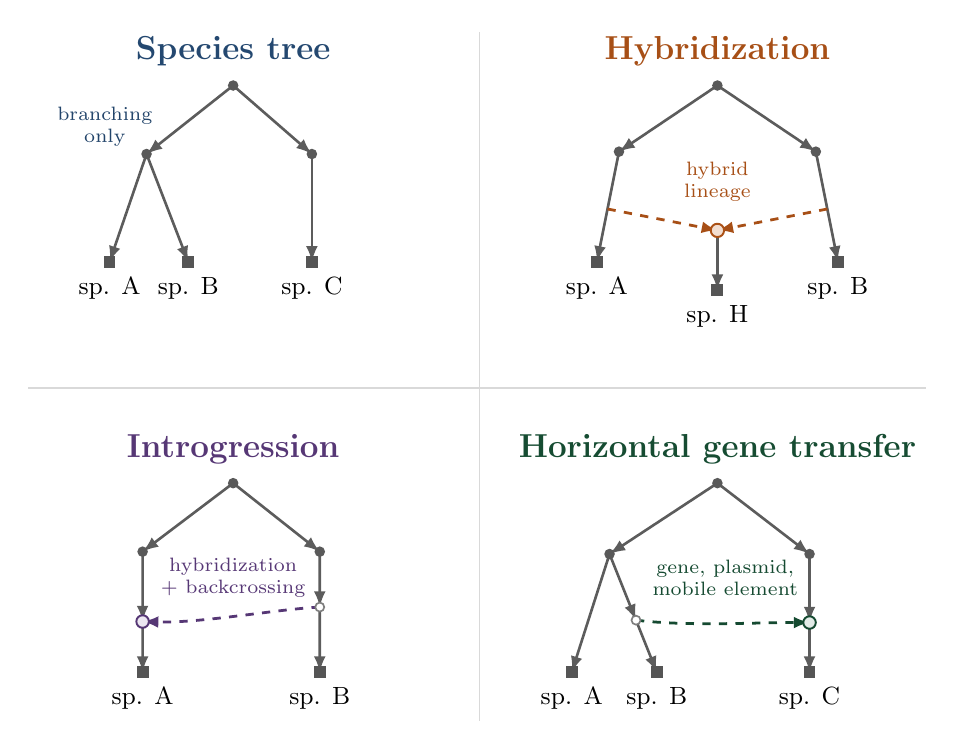
\begin{tikzpicture}[
  scale=1.0,
  paneltitle/.style={font=\bfseries\large},
  speciesedge/.style={-{Latex[length=2mm]},line width=.95pt,draw=darkgray!88,line cap=round},
  hybridedge/.style={-{Latex[length=2mm]},line width=1.0pt,dashed,draw=burntorange!88!black},
  introedge/.style={-{Latex[length=2mm]},line width=1.0pt,dashed,draw=violet!78!black},
  hgtedge/.style={-{Latex[length=2mm]},line width=1.0pt,dashed,draw=deepgreen!70!black},
  inode/.style={circle,fill=darkgray!90,inner sep=1.35pt},
  tipmark/.style={rectangle,fill=darkgray!92,inner sep=2.15pt},
  hybridnode/.style={circle,draw=burntorange!90!black,fill=burntorange!20,line width=.7pt,inner sep=1.7pt},
  intronode/.style={circle,draw=violet!78!black,fill=violet!13,line width=.7pt,inner sep=1.6pt},
  hgtnode/.style={circle,draw=deepgreen!70!black,fill=deepgreen!13,line width=.7pt,inner sep=1.6pt},
  sourcepoint/.style={circle,draw=darkgray!70,fill=white,line width=.6pt,inner sep=1.15pt},
  callout/.style={font=\scriptsize,align=center,text=darkgray},
  paneltext/.style={font=\small,align=center,text width=5.35cm,text=darkgray}
]

\begin{scope}
  \node[paneltitle,text=mainblue!85!black] at (2.45,3.45)
    {Species tree};

  \coordinate (r)  at (2.45,3.02);
  \coordinate (n1) at (1.35,2.15);
  \coordinate (n2) at (3.45,2.15);
  \coordinate (A)  at (0.88,0.78);
  \coordinate (B)  at (1.88,0.78);
  \coordinate (C)  at (3.45,0.78);

  \draw[speciesedge] (r)--(n1);
  \draw[speciesedge] (r)--(n2);
  \draw[speciesedge] (n1)--(A);
  \draw[speciesedge] (n1)--(B);
  \draw[speciesedge] (n2)--(C);

  \foreach \p in {r,n1,n2}{
    \node[inode] at (\p) {};
  }

  \foreach \p/\lab in {A/A,B/B,C/C}{
    \node[tipmark] at (\p) {};
    \node[below=2pt,font=\small] at (\p) {sp. \lab};
  }

  \node[callout,text=mainblue!80!black] at (0.82,2.50)
    {branching\\only};
\end{scope}

\begin{scope}[xshift=6.15cm]
  \node[paneltitle,text=burntorange!88!black] at (2.45,3.45)
    {Hybridization};

  \coordinate (r)  at (2.45,3.02);
  \coordinate (l)  at (1.20,2.18);
  \coordinate (rr) at (3.70,2.18);
  \coordinate (A)  at (0.92,0.78);
  \coordinate (B)  at (3.98,0.78);

  \coordinate (leftParent)  at ($(l)!0.52!(A)$);
  \coordinate (rightParent) at ($(rr)!0.52!(B)$);
  \coordinate (h) at (2.45,1.18);
  \coordinate (H) at (2.45,0.42);

  \draw[speciesedge] (r)--(l);
  \draw[speciesedge] (r)--(rr);
  \draw[speciesedge] (l)--(A);
  \draw[speciesedge] (rr)--(B);

  \draw[hybridedge] (leftParent)--(h);
  \draw[hybridedge] (rightParent)--(h);
  \draw[speciesedge] (h)--(H);

  \foreach \p in {r,l,rr}{
    \node[inode] at (\p) {};
  }

  \node[hybridnode] at (h) {};

  \foreach \p/\lab in {A/A,B/B,H/H}{
    \node[tipmark] at (\p) {};
    \node[below=2pt,font=\small] at (\p) {sp. \lab};
  }

  \node[callout,text=burntorange!88!black] at (2.45,1.80)
    {hybrid\\lineage};
\end{scope}

\draw[gray!30,line width=.55pt] (-0.15,-0.82)--(11.25,-0.82);

\begin{scope}[yshift=-5.05cm]
  \node[paneltitle,text=violet!78!black] at (2.45,3.45)
    {Introgression};

  \coordinate (r)  at (2.45,3.02);
  \coordinate (l)  at (1.30,2.15);
  \coordinate (rr) at (3.55,2.15);
  \coordinate (A)  at (1.30,0.62);
  \coordinate (B)  at (3.55,0.62);

  \coordinate (donor)     at ($(rr)!0.46!(B)$);
  \coordinate (recipient) at ($(l)!0.58!(A)$);

  \draw[speciesedge] (r)--(l);
  \draw[speciesedge] (r)--(rr);
  \draw[speciesedge] (l)--(recipient);
  \draw[speciesedge] (recipient)--(A);
  \draw[speciesedge] (rr)--(donor);
  \draw[speciesedge] (donor)--(B);

  \draw[introedge]
    (donor) .. controls (3.00,1.42) and (2.05,1.24) .. (recipient);

  \foreach \p in {r,l,rr}{
    \node[inode] at (\p) {};
  }

  \node[sourcepoint] at (donor) {};
  \node[intronode] at (recipient) {};

  \foreach \p/\lab in {A/A,B/B}{
    \node[tipmark] at (\p) {};
    \node[below=2pt,font=\small] at (\p) {sp. \lab};
  }

  \node[callout,text=violet!78!black] at (2.45,1.82)
    {hybridization\\+ backcrossing};
\end{scope}

\begin{scope}[xshift=6.15cm,yshift=-5.05cm]
  \node[paneltitle,text=deepgreen!72!black] at (2.45,3.45)
    {Horizontal gene transfer};

  \coordinate (r)  at (2.45,3.02);
  \coordinate (l)  at (1.08,2.12);
  \coordinate (rr) at (3.62,2.12);
  \coordinate (A)  at (0.60,0.62);
  \coordinate (B)  at (1.68,0.62);
  \coordinate (C)  at (3.62,0.62);

  \coordinate (donor)     at ($(l)!0.56!(B)$);
  \coordinate (recipient) at ($(rr)!0.58!(C)$);

  \draw[speciesedge] (r)--(l);
  \draw[speciesedge] (r)--(rr);
  \draw[speciesedge] (l)--(A);
  \draw[speciesedge] (l)--(donor);
  \draw[speciesedge] (donor)--(B);
  \draw[speciesedge] (rr)--(recipient);
  \draw[speciesedge] (recipient)--(C);

  \draw[hgtedge]
    (donor) .. controls (2.08,1.20) and (2.88,1.25) .. (recipient);

  \foreach \p in {r,l,rr}{
    \node[inode] at (\p) {};
  }

  \node[sourcepoint] at (donor) {};
  \node[hgtnode] at (recipient) {};

  \foreach \p/\lab in {A/A,B/B,C/C}{
    \node[tipmark] at (\p) {};
    \node[below=2pt,font=\small] at (\p) {sp. \lab};
  }

  \node[callout,text=deepgreen!70!black] at (2.55,1.82)
    {gene, plasmid,\\mobile element};
\end{scope}

\draw[gray!30,line width=.55pt] (5.58,-5.05)--(5.58,3.70);

\end{tikzpicture}
\end{document}
